\chapter{Method}

The method for our controlled experiment mimics Fucci et al.~\cite{fucci_replication_2019} with some differences: We have reimplemented the task in eeg-notebooks, used a different device, and have a smaller \& less diverse sample.

We start by deciding on an EEG device to use, then we collect data for both the controlled and organic experiments.

Once data collection is done, we continue with our analysis by training classifiers using various machine learning methods.

\begin{figure}[h]
    \begin{center}
        \includegraphics[width=10cm]{img/method.png}
    \end{center}
    \caption{Overview of the process for the two seperate tasks}\label{fig:method}
\end{figure}

\pagebreak

% Equipment
\section{Devices}
    
    In this section we will briefly describe the different EEG devices we have worked with, and their differences.

    We experimented with several devices but eventually settled on the Muse S. The motivation for choosing the Muse S was mainly due to comfort and ease of use. 

    The other devices considered included the OpenBCI Cyton (with the Ultracortex headset), and the Neurosity Crown.\footnote{Earlier in the work, before we received the Crown, we were also generously gifted a Neurosity Notion DK1 to get a head start.} 

    We have tried to make the code support all of the headsets mentioned (and more), such that future work can use whichever device one wants.

    \vspace{0.5cm}

    \begin{table}[H]
        \centering
        \begin{tabular}{llccc}
            \toprule
            Manufacturer
            & Device
            & Channels
            & Sampling rate
            & Comfort
            \\
            \midrule
            InteraXon
            & Muse S
            & 4
            & 256Hz
            & High \\
         OpenBCI
            & Cyton (with Ultracortex)
            & 8--16
            & 125--250Hz
            & Low \\
          Neurosity
            & Crown
            & 8
            & 256Hz
            & Medium \\
            \bottomrule
        \end{tabular}
        \caption{Devices used}\label{table:devices}
    \end{table}

    \vspace{0.5cm}

    \begin{minipage}{\textwidth}
        \paragraph*{Muse S}
        The Muse S is a 4-channel EEG headband with electrodes at TP9, AF7, AF8, and TP10, with the reference electrode at Fpz~\cite{krigolson_choosing_2017}. Its main advantage is its perfect comfort and long battery life. It's limited by its channel count and electrode placement. It connects using Bluetooth.

        \begin{figure}[H]
            \centering
            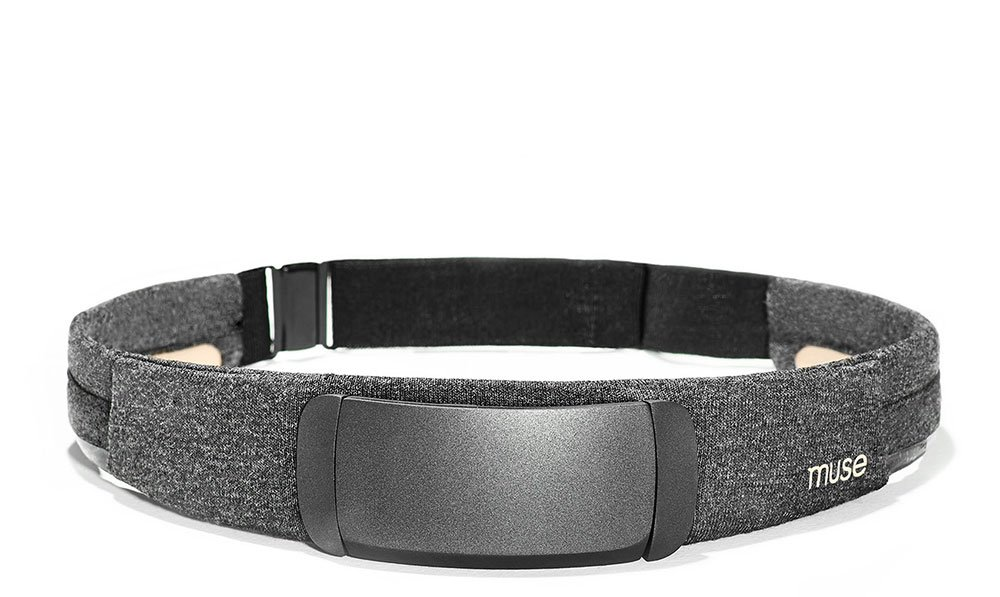
\includegraphics[trim=0 0 0 200,clip,width=100mm]{img/Muse-S.jpg}
            \caption{Muse S}\label{fig:museS}
        \end{figure}
    \end{minipage}

    \begin{minipage}{\textwidth}
        \paragraph*{OpenBCI Cyton}
        The OpenBCI Cyton is a 8-channel EEG board. It is commonly used with the partly 3D-printable OpenBCI Ultracortex headset, which allows for flexible electrode placement. OpenBCI also offers an expansion board, the Daisy, which adds 8 additional channels. It connects using Bluetooth.

        %The main disadvantage is the comfort of the Ultracortex headset, which makes it difficult to use for longer sessions. A wet-cap headset would address this, but that has other disadvantages, like being messy and time-consuming.

        \begin{figure}[H]
            \centering
            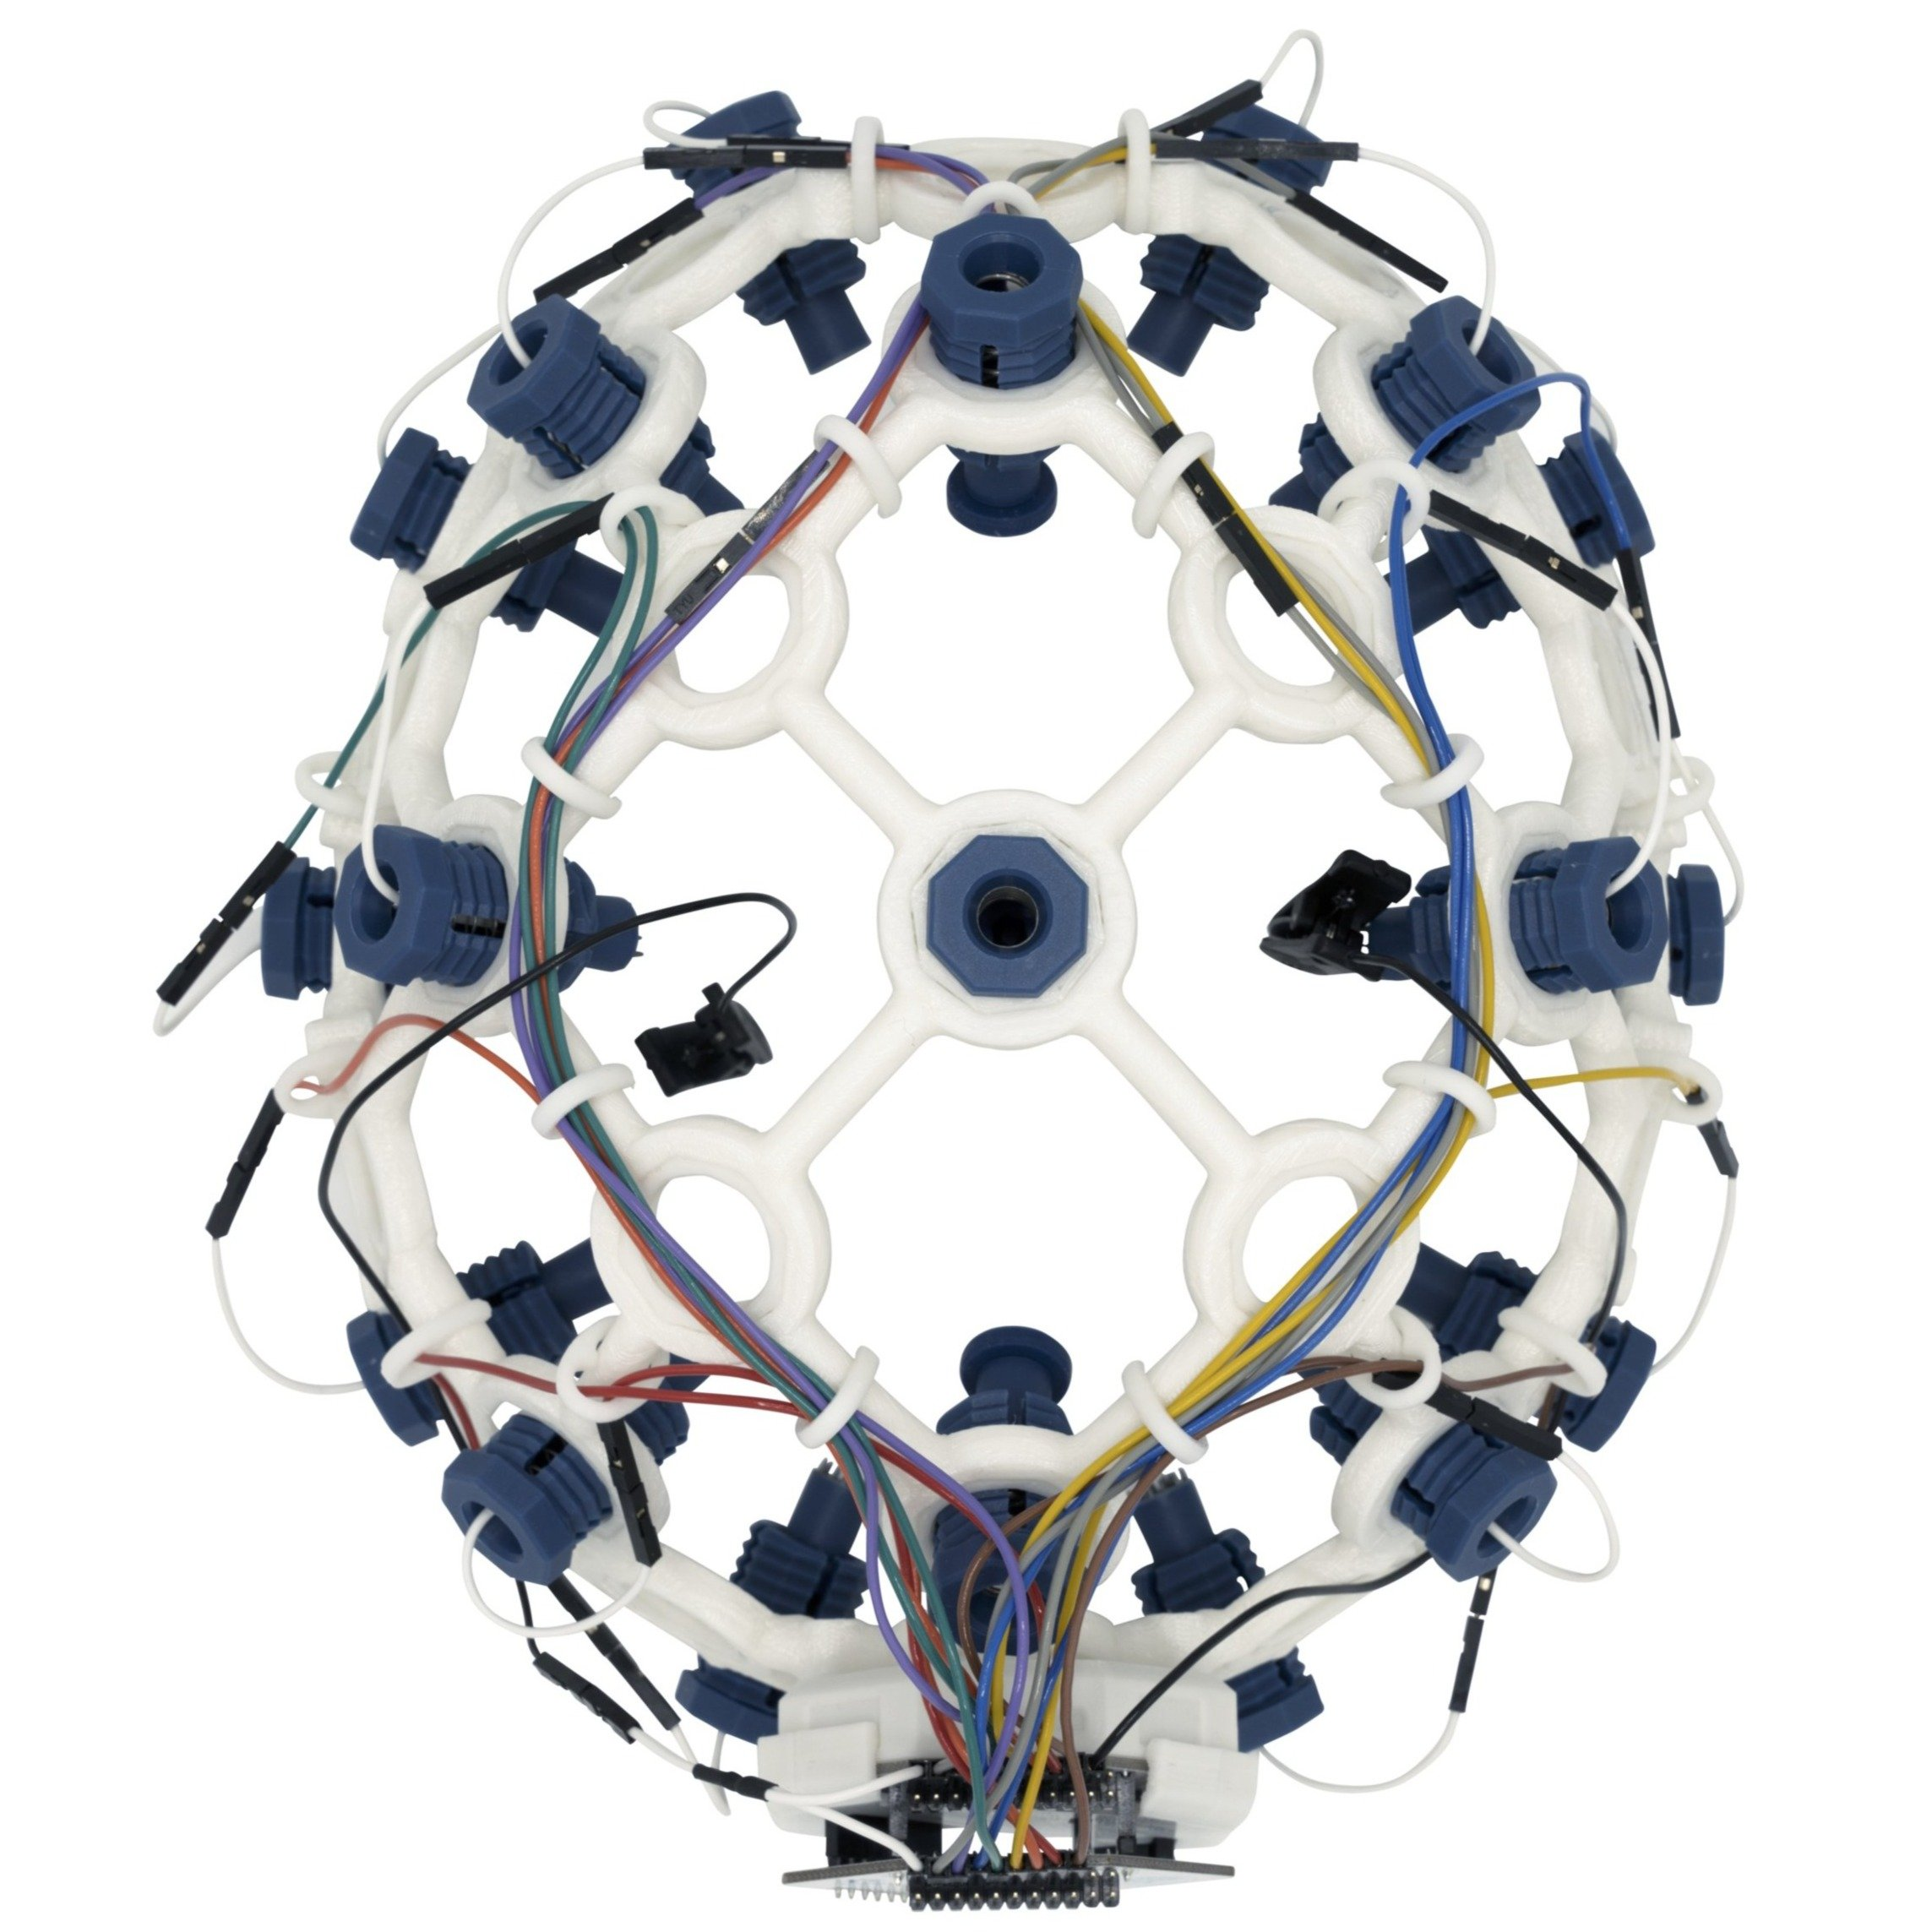
\includegraphics[width=80mm]{img/openbci-cyton.jpg}
            \caption{OpenBCI Cyton + Daisy with Ultracortex}\label{fig:cyton}
        \end{figure}
    \end{minipage}

    \vspace{1cm}

    \begin{minipage}{\textwidth}
        \paragraph*{Neurosity Crown}
        The Neurosity Crown is a 8-channel EEG headset. It runs Linux on a quad-core CPU and 1GB RAM, and connects via WiFi. It has electrodes placed at CP3, C3, F5, PO3, PO4, F6, C4, CP4. Reference and bias electrodes at T7 and T8.

        \begin{figure}[H]
            \centering
            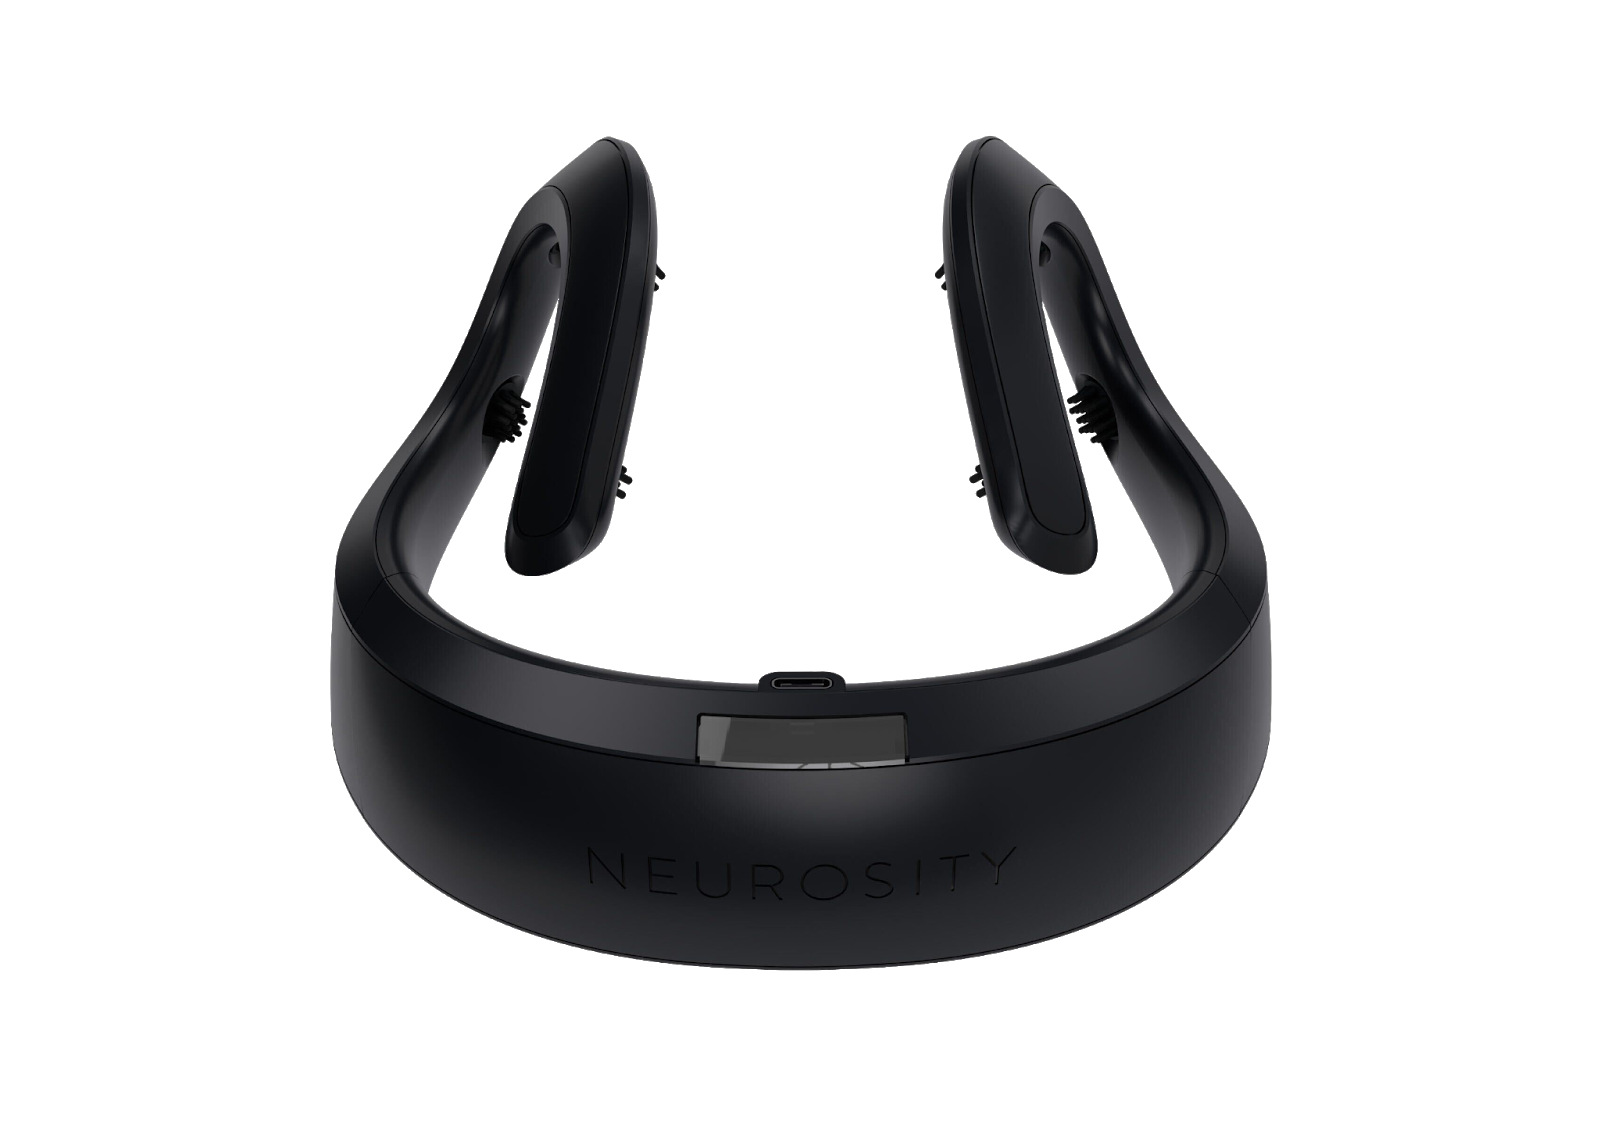
\includegraphics[trim=0 100 0 100,clip,width=100mm]{img/crown-1.png}
            \caption{Neurosity Crown}\label{fig:crown}
        \end{figure}
    \end{minipage}

\pagebreak
\section{Collection}

We need two types of data for the experiments: EEG data, and labels.

To collect data for the organic use experiment, we:

\begin{enumerate}
    \item Set up the EEG equipment
    \item Configure ActivityWatch to collect device usage data
\end{enumerate}

To collect data for the controlled experiment, we:

\begin{enumerate}
    \item Set up the EEG equipment
    \item Use eeg-notebooks to present the stimuli, and record the time markers of when the stimuli changed as labels.
\end{enumerate}

    \subsection{Collection of EEG data}

        EEG data was collected during organic device use and under controlled conditions.

        For both conditions, code from the open source eeg-notebooks~\cite{barachant_eeg-notebooks_2020} was adapted to record the raw EEG stream into a CSV file.

        Depending on the device used we require certain software to connect to the devices. We used muse-lsl for the Muse S~\cite{muse-lsl} which in turn uses Lab Streaming Layer. To support OpenBCI and Neurosity devices we used brainflow~\cite{noauthor_brainflow_2020}.

        We have developed `brainwatch', a command-line interface tool, to help us connect to and record from EEG devices. To connect \& record from an EEG device, we can simply run:

\begin{minted}{bash}
brainwatch connect --device museS

Searching for Muses, this may take up to 10 seconds...
Found device MuseS-2754, MAC Address 00:55:DA:B9:27:54
Recording to recording_2021-09-29-09.22.24.csv
\end{minted}

        We can then check signal quality with: \mintinline{bash}{brainwatch check}

        Or run the following to plot the raw signal: \mintinline{bash}{brainwatch plot}

        Alternatively, we can plot using muse-lsl's built-in plotting functionality: \mintinline{bash}{muselsl view -b Qt5Agg}

        \begin{sidewaysfigure}
            \begin{center}
                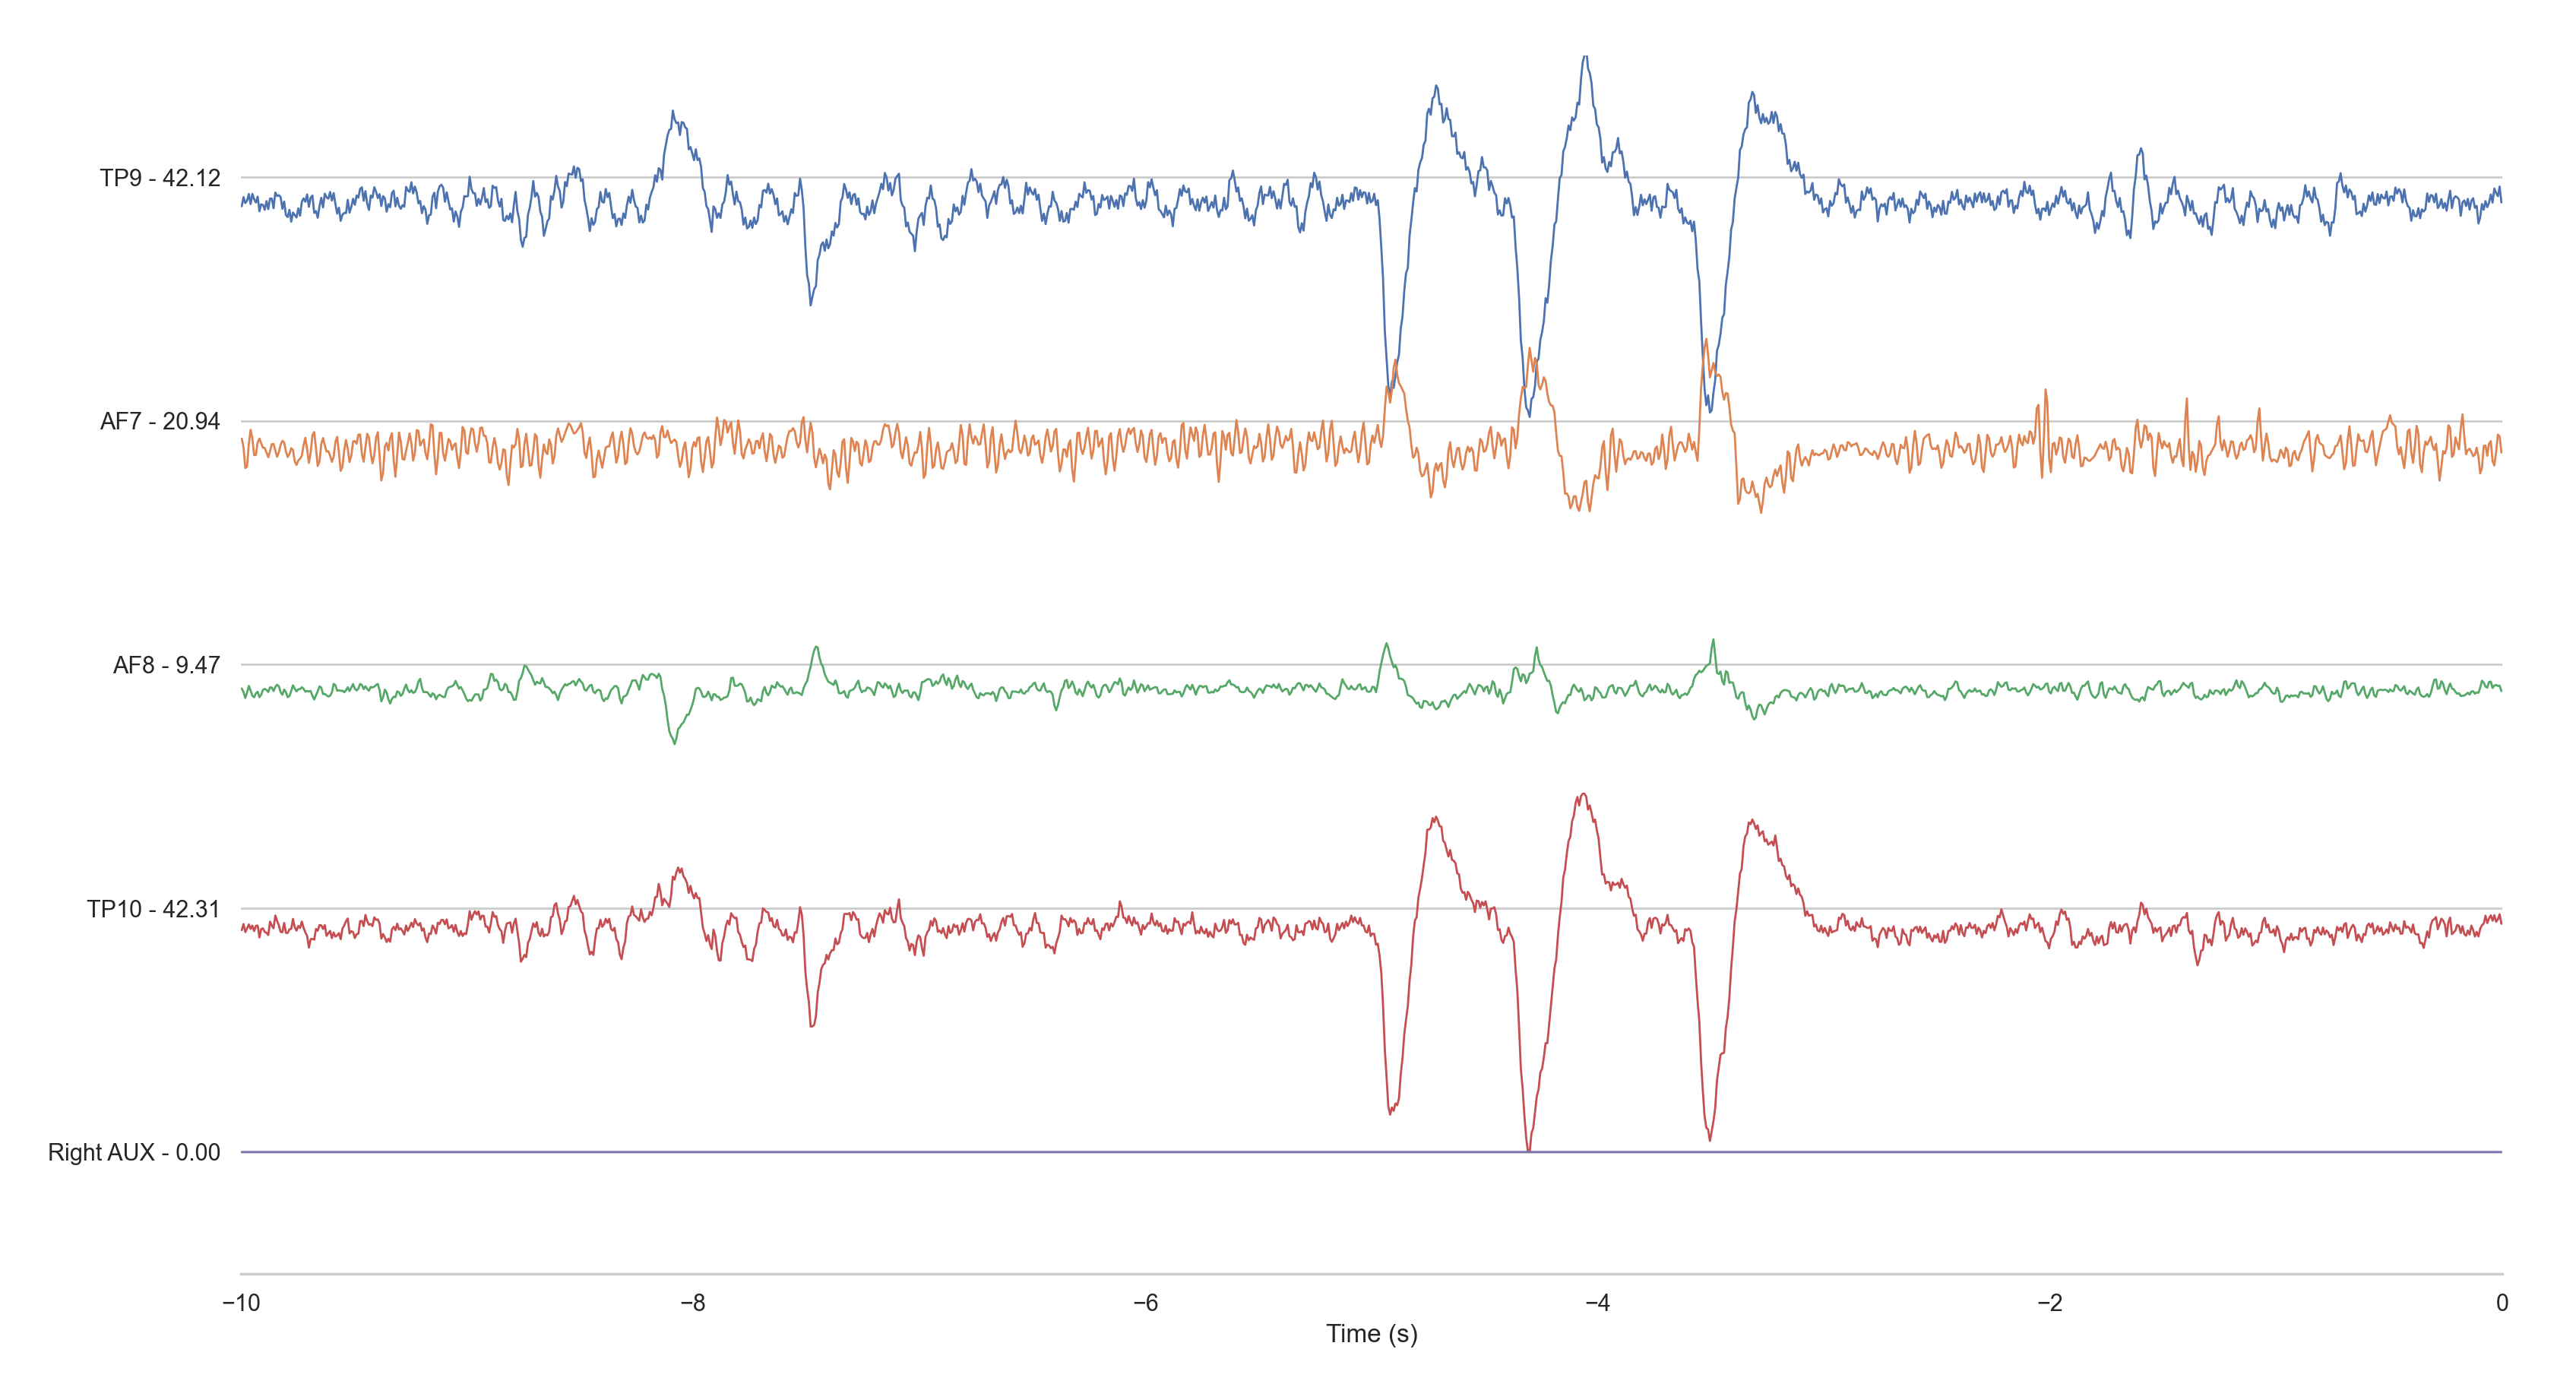
\includegraphics[trim=60 50 50 60,clip,width=24cm]{img/raw-signal.png}
            \end{center}
            \caption{EEG signal, with 3 eye blinks identifiable around $\SI{-4}{\second}$.\\ The signal has been bandpass filtered to eliminate noise.}\label{fig:raweeg}
        \end{sidewaysfigure}

        \subsubsection*{During organic device use}

            For the organic device use conditions, we used the Muse S due the superior comfort and ease of use compared with the alternatives, making it especially suitable for long recordings.\footnote{A wet electrode cap system was also considered, but ultimately not investigated due to being inconvenient to setup.}

            For this experiment we use a single-subject, with the experimenter as the subject.

            The subject was asked to go about their usual device activities, often consisting of a mix of work (email, writing prose, writing code) and leisure (watching YouTube, reading Twitter).

        \subsubsection*{During code vs prose comprehension task}

            For the controlled condition, we ended up using the Muse S as well due to the comfort and ease of setup.

            We have 9 subjects, sampled by convenience. The subjects were 8 males and one female. Most are in their late 20s or early 30s, except two who are in their 40s.

            The experiment consists of presenting images with code or prose comprehension tasks, as seen in Figure~\ref{fig:codetask} and~\ref{fig:prosetask}. These images are from previous studies on code vs prose comprehension by Floyd et al~\cite{floyd_decoding_2017} and Fucci et al.\cite{fucci_replication_2019}. We note that Fucci et al. modified the prose comprehension images from the original review-like task to become more comprehension-like, arguably better suited for the task. However, due to the images being in Italian, we've used the original images used by Floyd et al.

            We implemented the task in eeg-notebooks~\cite{barachant_eeg-notebooks_2020}, which uses previously mentioned libraries for data collection as well as PsychoPy~\cite{peirce_psychopy2_2019} to provide the stimuli.

            \begin{figure}[h]
                \begin{center}
                    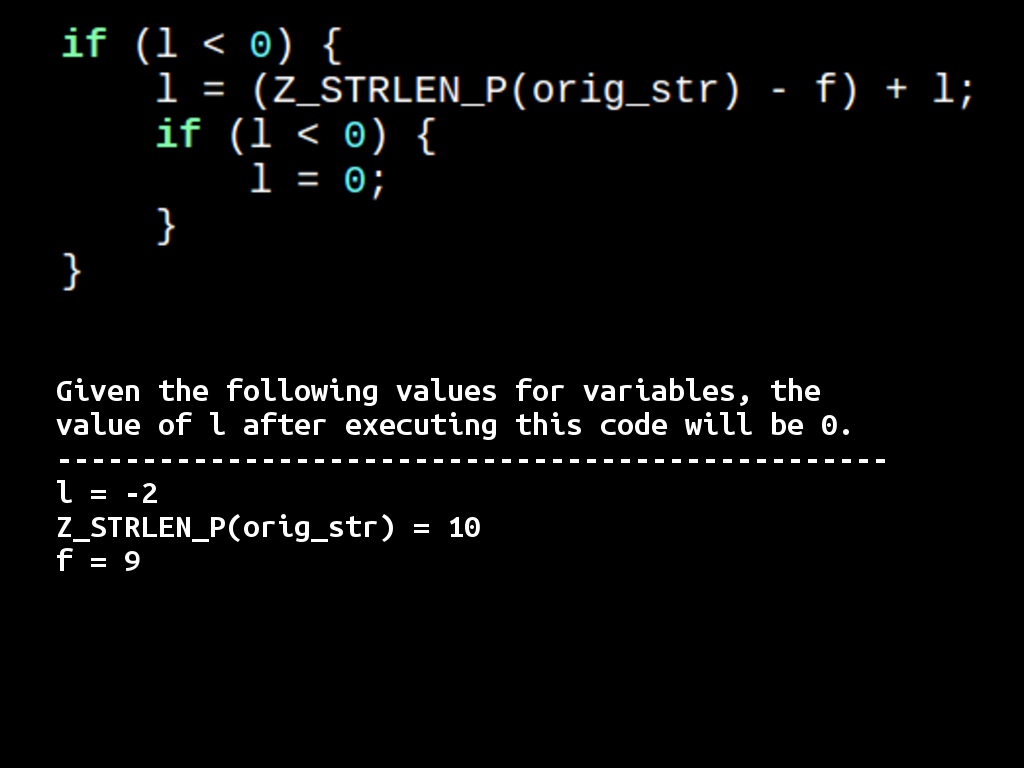
\includegraphics[trim=0 120 0 0,clip,width=100mm]{img/final-1-1.png}
                \end{center}
                \caption{Sample of the code comprehension task}\label{fig:codetask}
            \end{figure}

            \begin{figure}[h]
                \begin{center}
                    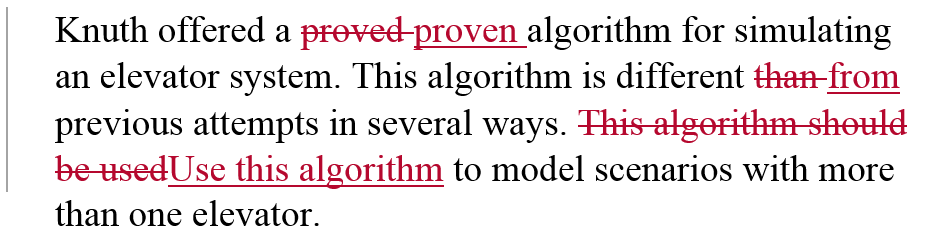
\includegraphics[width=100mm]{img/bugs_1.PNG}
                \end{center}
                \caption{Sample of the prose review task}\label{fig:prosetask}
            \end{figure}

            Before each run, the subject was asked about their gender, age, and software development experience (specifically experience with C/C++). For good measure, we also asked if the subject had consumed caffeine the hours prior to the experiment.

            After these questions we put the devices on and ensure we get good signal by inspecting it in real time with the viewer provided by muse-lsl. The viewer itself does simple bandpass filtering between 3--40Hz, and the signal quality is indicated by the standard deviation of the filtered signal.

    \subsection{Collection of device activity data}

        All device activity is collected using the automated time tracker ActivityWatch~\cite{bjareholt_activitywatch_2020-1}.

        ActivityWatch collects data through modules called watchers which report to the ActivityWatch server. It comes with two watchers by default:

        \begin{itemize}
            \item aw-watcher-window, tracks the active window and its title
            \item aw-watcher-afk, tracks if the user is active or not by observing input device activity
        \end{itemize}

        We have also built a custom watcher, aw-watcher-input, to track metrics of mouse and keyboard activity. It tracks by listening to mouse and keyboard events and records the distance\footnote{in pixels} the mouse moves and number of clicks (but not which key was clicked). Every second this is bundled into an event, the values are reset, and then it continues with the next event. It was inspired by similar functionality in Andrej Karpathy's ulogme~\cite{karpathy_ulogme_2016}.

        A limitation that we have to consider is that the window watcher uses a polling method to track the active window, with a default poll time of 1 second. This means that we can't rely on the timestamps to mark the exact time the window became active/inactive.

        The data from ActivityWatch is processed and categorized such that the resulting data has the 3 columns \mintinline{text}{start, stop, class}. The class is determined by a regular expression that matches on window titles and URLs. For example, the regular expression \mintinline{text}{GitHub|github.com} could be used to match GitHub use.

\begin{figure}[h]
\begin{minted}{text}
start,               stop,                class
2020-09-20 13:07:41, 2020-09-20 13:08:20, YouTube
2020-09-20 13:32:51, 2020-09-20 13:34:09, Twitter
2020-09-20 14:44:08, 2020-09-20 14:46:11, YouTube
2020-09-21 09:49:04, 2020-09-21 09:49:35, GitHub->Issues
2020-09-21 09:51:32, 2020-09-21 09:52:23, YouTube
2020-09-21 10:04:29, 2020-09-21 10:05:01, GitHub->Issues
2020-09-21 10:20:18, 2020-09-21 10:21:05, Editing->Prose
\end{minted}
    \caption{Examples of labeled time windows, collected and categorized with ActivityWatch}\label{code:class-csv}
\end{figure}

\section{Analysis}

    For classification and analysis, we used common open source Python libraries for data analysis, like numpy~\cite{harris2020array}, pandas~\cite{reback2020pandas}, and scikit-learn~\cite{scikit-learn}. In addition, we used less common libraries tailored specifically for working with EEG data, such as MNE~\cite{noauthor_mne-python_2020}, pyriemann~\cite{alexandre_barachant_2020_3715511}, and YASA~\cite{vallat_yasa_2020}.

    \subsection{Labelling}
        For the organic device use experiment, we split the EEG data into epochs using the categories assigned by our ActivityWatch script.

        For the controlled experiment, we split the EEG data into epochs using the trial markers, resulting in one epoch per stimuli.

    \subsection{Data transformation}

        In order to train on the variable-length epochs, we need to split each epoch into a fixed-duration window, which can then be used to train and classify our model.

        Dimensions of each epoch matrix: \[ (n_{samples}, n_{channels}) \]

        Where $n_{samples}$ is the total number of samples for the epoch (variable-length), and $n_{channels}$ is 4 for the Muse S.

        Since the matrix has variable dimensions for each epoch, we split it into $\sim$5s windows, which at the 256Hz sampling frequency of the Muse gives us 1280 samples per window.

        Dimensions of the window matrix: \[ (n_{windows}, n_{channels}, 1280) \]

        We experimented with different windowing methods to potentially augment the data...  \todo[inline]{...and? Should a sliding window approach be used to improve data augmentation?}

    \subsection{Data cleaning}

        % TODO: Should this say 'reject windows' instead?
        We reject samples that either:

        \begin{enumerate}
            \item Don't have an assigned class
            \item Have a bad signal quality (as indicated by a high signal variance)
            \item Are too short (due to missing samples)
        \end{enumerate}

        \todo[inline]{List how many epochs are rejected by each cleaning step}

    \subsection{Feature engineering}

        One approach to classifying EEG data is to perform feature extraction/engineering. Common features used for EEG data include bandpower ratios, as well as covariance matrixes using the Riemannian metric.

        To evaluate most common machine learning classifiers, we need to

        \subsubsection{Bandpower}

            \todo[inline]{Refer/move to theory section instead?}

            Bandpower features are simple and commonly used in EEG research for many tasks, including the paper by Fucci et al we seek to improve upon~\cite{fucci_replication_2019}. As a reference, we implemented classifiers which solely used bandpower features as input, to gain information of how much any improvement from classifier performance is likely due to better EEG equipment versus how much is due to from improved analysis methods.

            To compute this feature, we utilized the bandpower function provided by YASA~\cite{vallat_yasa_2020}. The implementation estimates the power spectral density using Welch's method for each channel, and bins them by their associated frequency band.

            To further enrich our feature vector, we can use ratios between two frequency bands.

        \subsubsection{Riemannian geometry}

            \todo[inline]{Refer/move to theory section instead?}

            The \improvement{according to whom?}{state of the art in many EEG classification tasks} involves the use of Riemannian geometry. For this, we used the open source pyriemann library by Alexandre Barachant\footnote{First author of the original paper to apply Riemannian geometry to EEG~\cite{barachant_classification_2013}}.

    \subsection{Neural Networks}

        One of the classifiers we want to train is a neural network. We use braindecode~\cite{schirrmeister_deep_2017}\cite{noauthor_braindecode_2021}, a neural network toolbox for EEG data that uses PyTorch and integrates it with scikit-learn through skorch.

        The networks provided by braindecode are convolutional\ldots

    \subsection{Cross Validation}

        We use LORO (``Leave-One-Run-Out'') cross-validation, a variation of LOGO (``Leave-One-Group-Out''), in order to ensure the samples used in validation are using subjects or tasks that are unseen in training.

        We attempt both out-of-subject validation and out-of-task validation in order to estimate the ability of the classifiers to generalize across subjects and tasks.

    \subsection{Single subject}

        % TODO: what experiments?
        % TODO: what devices?
        % FIXME: is this out of scope?
        We experimented with single-subject analysis to validate different devices and tasks.
